\documentclass[a4paper,10pt]{article}
\usepackage[margin=1in]{geometry}
\usepackage{polski}
\usepackage[utf8x]{inputenc}
\usepackage[unicode]{hyperref}
\usepackage{amssymb}
\usepackage{xifthen}
\usepackage[fleqn]{amsmath}
\usepackage{todonotes}
\usepackage{graphicx}
\usepackage{float}
\usepackage{fullpage}
\usepackage{epstopdf}
\usepackage{multirow}
\usepackage{subfig}
\usepackage[europeanresistors,americaninductors]{circuitikz}
\usetikzlibrary{patterns}
\newcommand{\withtodo}{0}


\def\arraystretch{1.2}


\begin{document}

\begin{table}
  \centering
  \def\arraystretch{1.5}
    \begin{tabular}{|l|l|l|l|} \hline
    Wydział:           & \multicolumn{2}{l|}{Dzień:Poniedziałek 14-17}    &Zespół:  \\
    Fizyki             &    \multicolumn{2}{l|}{Data: 20.03.2017}         &8             \\\hline
    Imiona i nazwiska: &Ocena z przygotowania:  &Ocena ze sprawozdania:   &Ocena końcowa: \\
    Marta Pogorzelska  &                        &                         &                \\
    Paulina Marikin    &                        &                         &\\\hline
    \multicolumn{2}{|l|}{Prowadzący:                 } &\multicolumn{2}{l|}{Podpis:             }  \\\hline
  \end{tabular}
\end{table}

\title{Ćwiczenie 43:\\Wyznaczanie $\frac{c_p}{c_v}$ dla powietrza metodą rezonansu akustycznego}
\date{}
\maketitle

\section{Cel badań}
Doświadczenie miało na celu wyznaczenie współczynnika adiabaty dla powietrza.

\section{Wstęp teoretyczny}
$\kappa$ jest współczynnikiem w równaniu adiabaty, zależnym od ilości stopni swobody danego gazu. W modelu gazu doskonałego pomijane są drgania cząsteczek, zaś ich rotacja, dla cząstek jedno i dwu atomowych, nie wpływa znacząco na interakcje z otoczeniem i także jest pomijana. Definiowany jest on równaniami:

\begin{equation}
  \kappa = \frac{c_p}{c_V} = 1+\frac{1}{n}
\end{equation}
$c_p$ - ciepło własćiwe przy stałym ciśnieniu, $c_V$ - ciepło właściwe przy stałej objętości, n - liczba stopni swobody.
\\\\W tym doświadczeniu jege wartość dla powietrza została wyznaczona metodą Laplac'a, wiążącą równania terodynamiczne z zachowaniem fali akustycznej. Falą taką jest podłużna fala mechanicznaoscylująca w zakresie słyszalnym dla człowieka. Jej ruch to okresowa kompresja i dekompresja ośrodka zachodząca adiabatycznie, można więc do jego opisania stosować równanie adiabaty z którego, w połączeniu z równaniem
falowym i równaniem Clapeyrona otrzymujemy:

\begin{equation}
  \kappa = \frac{v^2 \rho}{p}
\end{equation}
Prędkość fali została zmierzona pośrednio na podstawie równości $v = \lambda f$ co wstawione do poprzedniego równania daje nam finalny wzór:
\begin{equation}
  \kappa = \frac{\lambda^2 f^2 M}{kT}
\end{equation}

\section{Opis układu i metody pomiarowej}
Użyte przyrządy:
\begin{itemize}
  \item oscyloskop z podłączonymi sygnałami od generatora i mikrofonu
  \item miarka z podziałką 1mm
  \item głośnik
  \item mikrofon na ruchomym tłoku
  \item rurka z plexi wypełniona powietrzem
  \item regulowany generator sygnału
	\item wzmacniacz sygnału
  \item termometr z podziałką $2^\circ C$
\end{itemize}
Oscyloskop został ustawiony na tryb X-Y pokazujący krzywą eliptyczną gdzie x to sygnał z generatora, a y z mikrofonu. W celu wyznaczenia kolejnych długości fali mierzone były odległości między kolejnymi węzłami, za które uznano maksymalne zwężenie krzywej eliptycznej do prostej. W celu uzyskania kolejnych  wezłów manipulowano tłokiem z doczepionym mikrofonem.
Zamiast okresu dla każdej z fal została zmierzona częstotliwość $\omega = 2 \pi T$, mierzona jako odległość między kolejnymi maksimami fali stojącje na
obrazie z oscyloskopu. Temperatura została zmierzona raz, po wykonaniu pozostałych pomiarów.

\section{Analiza pomiarów}

\begin{figure}[H]
  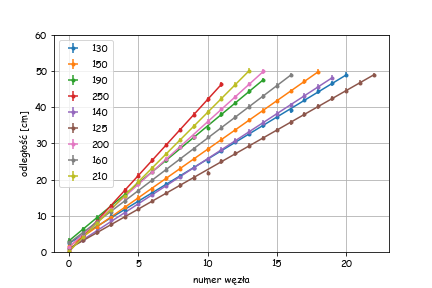
\includegraphics{./Kappa.png}
  \caption{wykres pozwalający wyliczyć długość fali}
  \label{}
\end{figure}
\begin{tabular}{lrrrrrrrrrr}
\toprule
{} &             k &             M &      T &  $\Delta$T &            f &  $\Delta$f &  $\lambda$ &  $\Delta \lambda$ &  $ \kappa$ &  $\Delta \kappa$ \\
{} & $\frac{J}{K} 10^{-23}$ & Kg $10^{-26}$ & K & K & Hz & Hz & m & m &&\\
\midrule
0 &  1.3806 &  4.81 &  299.0 &   1.3 &  8000.0000 &   0.0004 &   0.04352 &     0.00014 &   1.4120 &   0.0076 \\
1 &  1.3806 &  4.81 &  299.0 &   1.3 &  7692.3076 &   0.0003 &   0.04638 &     0.00015 &   1.4824 &   0.0081 \\
2 &  1.3806 &  4.81 &  299.0 &   1.3 &  7142.8571 &   0.0003 &   0.0496 &      0.00009 &   1.4644 &   0.0069 \\
3 &  1.3806 &  4.81 &  299.0 &   1.3 &  6666.66667 &   0.00028 &   0.0535 &      0.00008 &   1.4819 &   0.0068 \\
4 &  1.3806 &  4.81 &  299.0 &   1.3 &  6250.00000 &   0.00025 &   0.05785 &     0.00014 &    1.5226 &   0.0076 \\
5 &  1.3806 &  4.81 &  299.0 &   1.3 &  5263.15789 &   0.00017 &   0.06328 &     0.00025 &    1.2922 &   0.0076 \\
6 &  1.3806 &  4.81 &  299.0 &   1.3 &  5000.00000 &   0.00016 &   0.06896 &     0.00028 &    1.3849 &   0.0083 \\
7 &  1.3806 &  4.81 &  299.0 &   1.3 &  4761.90476 &   0.00014 &   0.0765 &      0.00004 &    1.5470 &   0.0067 \\
8 &  1.3806 &  4.81 &  299.0 &   1.3 &  4000.00000 &   0.00010 &   0.08376 &      0.00008 &    1.3076 &   0.0057 \\
\bottomrule
\end{tabular}
\section{Analiza niepewności}
Niepewności temperatury i okresu wyliczono z niepewności aparaturowych i eksperymentatora, zaś za niepewność długości fali został wzięty pierwiastek z kowariancji dopasowanej prostej. Niepewności częstotliwości i współczynnika adiabaty zostały wyznaczone przy użyciu metody propagacji niepewności.

\section{Wnioski}
Wszystkie wartości $\kappa$ są zbliżone do przewidywanego wyniku 1.4. Potwierdza to teoretyczne przewidywania dla modelu gazu doskonałego.
\\
Zjawisko rezonansu akustycznego pozwala na dokładne i łatwo wykonane wyznaczanie współczynnika adiabaty.Chociaż finalna niepewność jest relatywnie mała (poniżej 1\% wyniku) głównym czynnikiem ją generującym jest temperatura, której dokładność można łatwo poprawić używając lepszego termometru. Także, nieuwzględniane w opracowaniu zmiany temperatury w trakcie doświadczenia mogły prowadzić do odchyleń wyniku. Otrzymana na końcu $\kappa$ dla powietrza wynosi:
\\ $\kappa = 1.4311$\\


\end{document}
